\chapter{Anhang}

\section{Projektvereinbarung}
\label{projektvereinbarung}

\newpage

\section{Proof of Concept}
\label{poc}

Für die Einarbeitung in die Gephi-Plugin Entwicklung und erste Ansätze für die Umsetzung des Projekts zu finden, hat
sich das Projektteam entschlossen, ein Proof of Concept durchzuführen.

\subsection{Ziel}

Mit dem Proof of Concept, soll sich einerseits mit dem \ac{api} von \acs{gephi} vertraut zu machen.
Andererseits soll die Funktionsweise von ersten Ideen und Konzepten überprüft werden.

\subsection{Umsetzungsprozess}

\begin{itemize}
    \item \textbf{Filter:} Filter werden in \acs{gephi} verwendet, um ein Netzwerk auf Knoten oder Kanten zu reduzieren, welche bestimmte Eigenschaften besitzen.
    In Bezug auf Link-Prediction wurde deshalb eine neue Filterkategorie eingeführt, unter welcher nach verschiedenen Prediction-Algorithmen gefiltert werden kann.
    Durch Auswahl eines Algorithmus können jene Kanten herausgefiltert werden, welche durch Anwenden des Algorithmus neu hinzugefügt werden.
    Der Filter wird dabei um ein \acs{ui}-Element ergänzt, bei welchem die Anzahl der hinzugefügten Kanten eingegrenzt werden kann.

    \item \textbf{Statistiken:} Die Wahrscheinlinkteit, dass sich eine neue Kante zwischen zwei Knoten bildet, entspricht einem berechneten Wert.
    Diese Berechnung wird mittels Statistiken angestossen. Die gesamte Logik und Berechnung der verschiedenen Algorithmen wird anschliessend
    durch verschiedene Statistik-Objekte gekapselt.

    Die Funktionsweise für das Implementieren von neuen Statistik-Objekten ist im Gephi-Plugin Bootcamp gut dokumentiert. Darauf aufbauend
    konnte ein neues Statistik-Objekt mit entstprechendem Button im \acs{ui} implementiert werden. Bei der Berechnung wurde der Algorithmsu
    ``Common Neighbours'' eingesetzt, bei welchem die Anzahl Nachbarn jedes Knotens gezählt werden.

    Für die Implementierung des Algorithmus konnten bestehende Funktionen von \acs{gephi} verwendet werden um die Knoten aus dem Graphen, respektive
    dessen Nachbarn auszulesen. Die berechneten Werte konnten anschliessend bereits im \acs{datalaboratory} abgelegt werden.

    % TODO: Redundant?
    %Da für die Umsetzung der Link Prediction aber nicht nur die direkte Anzahl der Nachbarn relevant ist, sondern vor allem
    %die Zahl der gemeinsamen Nachbarn zweier Knoten wurde auch dafür noch eine Statistik umgesetzt. Hier werden nacheinander
    %die Knoten durchgegangen und getestet, wie viele ihrer Nachbarn mit den Nachbarn eines anderen Knotens übereinstimmen.
    %Wenn es noch keine Kante zwischen den beiden Knoten gibt, wird eine neue hinzugefügt und die Anzahl der gemeinsamen
    %Knoten als neues Attribut eingefügt. Wenn es die Kante bereits gibt, wird nur das neue Attribut befüllt. Zusätzlich
    %gibt es ein Attriut, das anzeigt, ob die Kante hinzugefügt wurde oder ob sie schon existiert hat. Zur Berechnung der
    %gemeinsamen Nachbarn werden darüber hinaus nur Kanten gewertet, die nicht erst bei der Berechnung hinzugefügt worden
    %sind.

    Damit dem Graphen Kanten hinzugefügt werden können, während diese noch gelesen und überarbeitet werden, muss ein Write-Lock
    verwendet werden. Die Logik, welche für den Algorithmus ``Common Neighbours'' implementiert wurde, kann für die spätere Umsetzung
    grösstenteils wiederverwendet werden.
\end{itemize}

\subsection{Erkenntnisse}

Es konnten verschiedene Erkenntnisse aus der Umsetzung des Proof Of Concept gewonnen werden.
Zum einen war es sehr hilfreich, sich zum ersten Mal aktiv mit dem \acs{api} von \acs{gephi} zu beschäftigen. Besonders wichtig war
dabei die Erkenntnis, dass die Beispiele aus dem Bootcamp teilweise veraltet sind. Um solche Beispiele mit einer neuen \acs{gepi}-Version
und den dadurch unterschiedlichen \acs{API}s zum Laufen zu bringen, muss zusätzlich Aufwand eingerechnet werden.

Weiter konnte mithilfe des Proof Of Concepts sichergestellt werden, dass sämtliche Installationen, Konfigurationen und die
Entwicklungsumgebung korrekt funktionieren. Viele konfigurative Probleme konnten hier bereits erkannt und frühzeitig behoben werden.

Vom technischen Aspekt her konnten wichtige Erkenntnisse für die spätere Umsetzung gewonnen werden - beispielsweise
wie ein Gephi-Plugin aufgebaut ist. Diese Erkenntnisse fliessen direkt in die Überlegungen beim Entwurf der Software-Architektur ein.
% TODO: Redundant?
%Um ein Beispiel zu nennen, konnte nach der Umsetzung des
%Proof of Concept aber bereits festgelegt werden, wie sichergestellt werden kann, dass die Anzahl Algorithmen für die
%Link Prediction beliebig erweitert werden kann, nämlich indem diverse Informationen in separate Klassen ausgelagert
%werden und es für jeden Algorithmus eine eigene Subklasse gibt, die grundsätzlich nur noch die Umsetzung des Algorithmus
%implementiert, jedoch nichts mit dessen Aufruf zu tun hat.
\newpage

\section{README.md}
\label{readme}

% Split readme in 3 parts
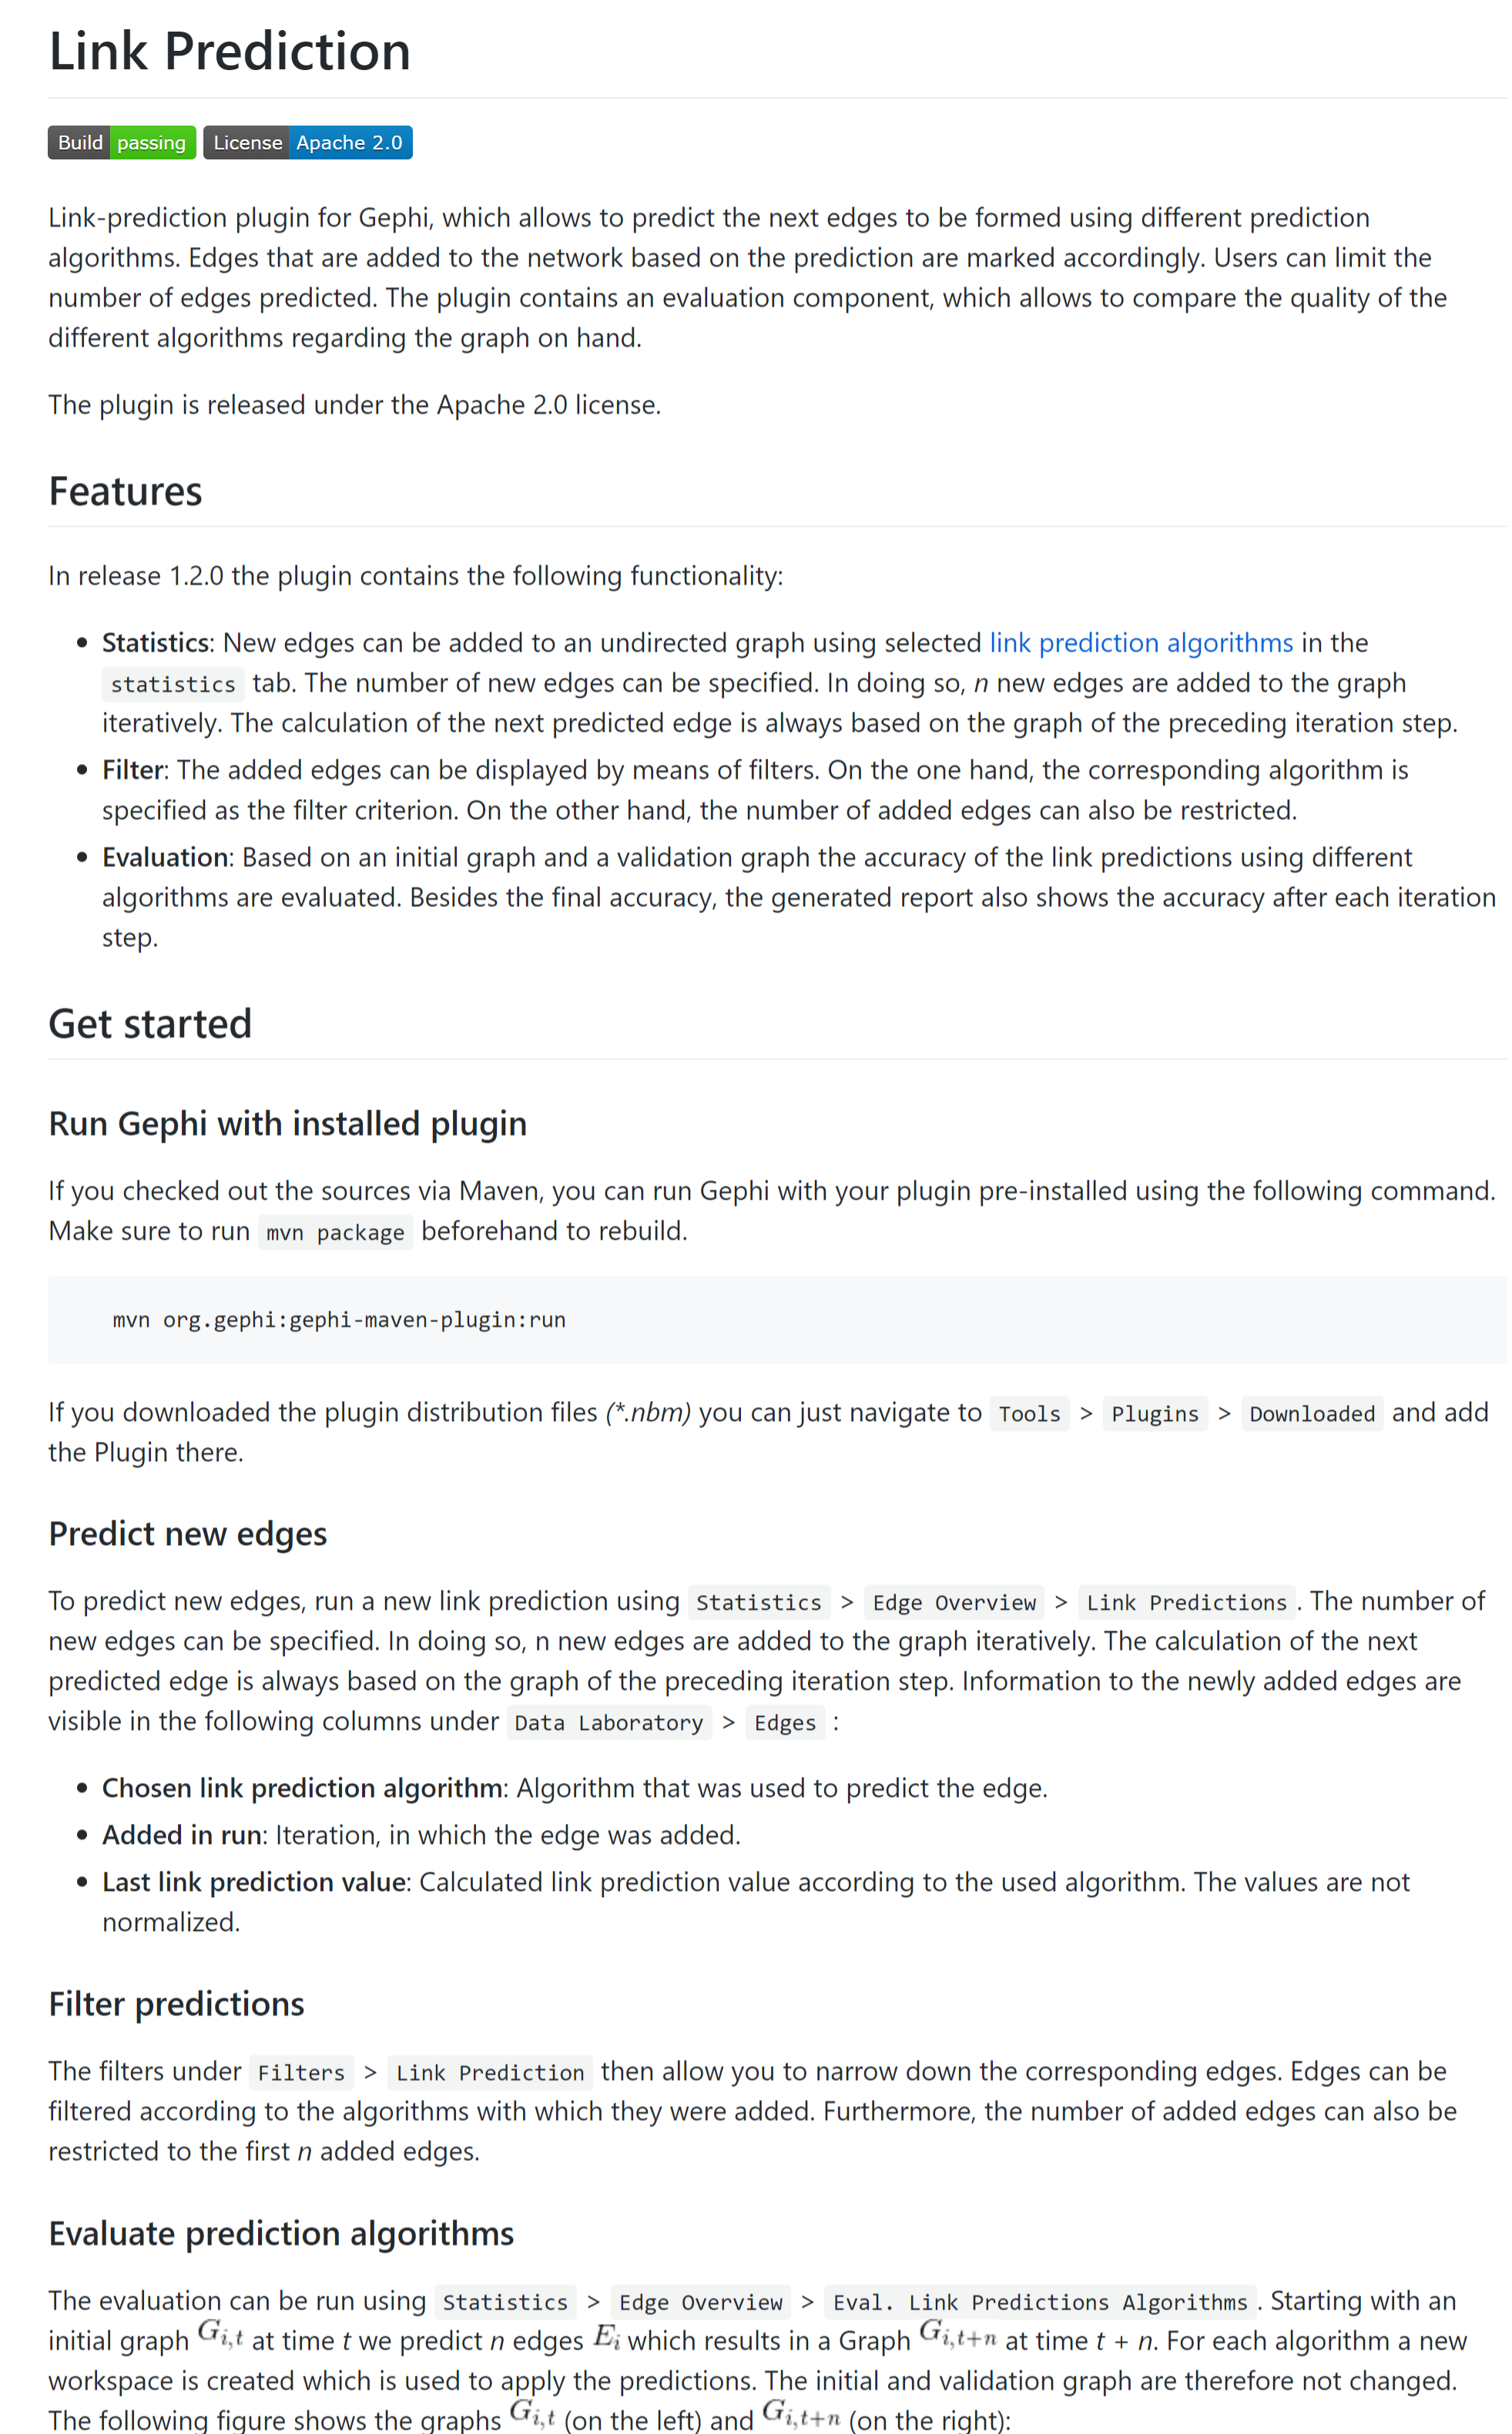
\includegraphics[width=\textwidth]{resources/readme_pt1.png}
\newpage
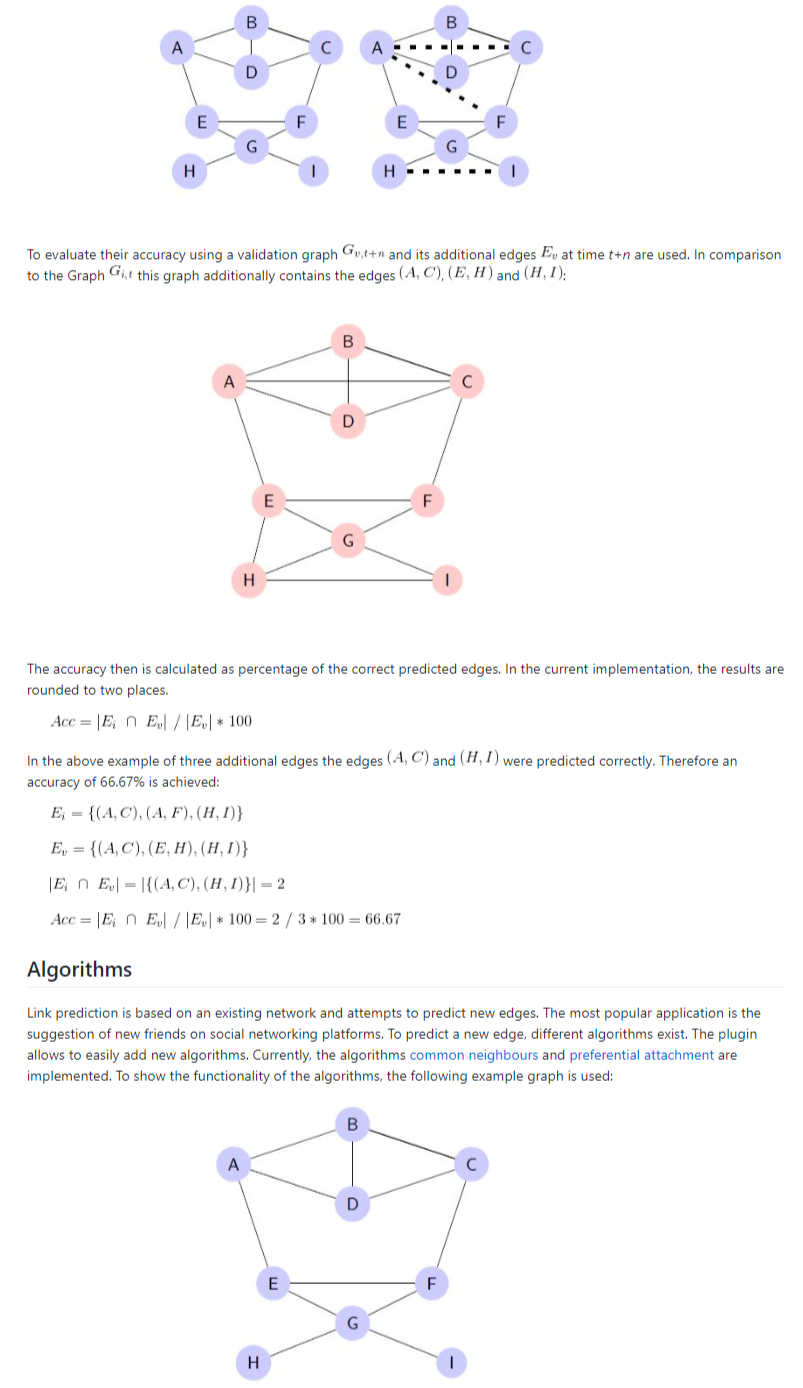
\includegraphics[width=\textwidth]{resources/readme_pt2.png}
\newpage
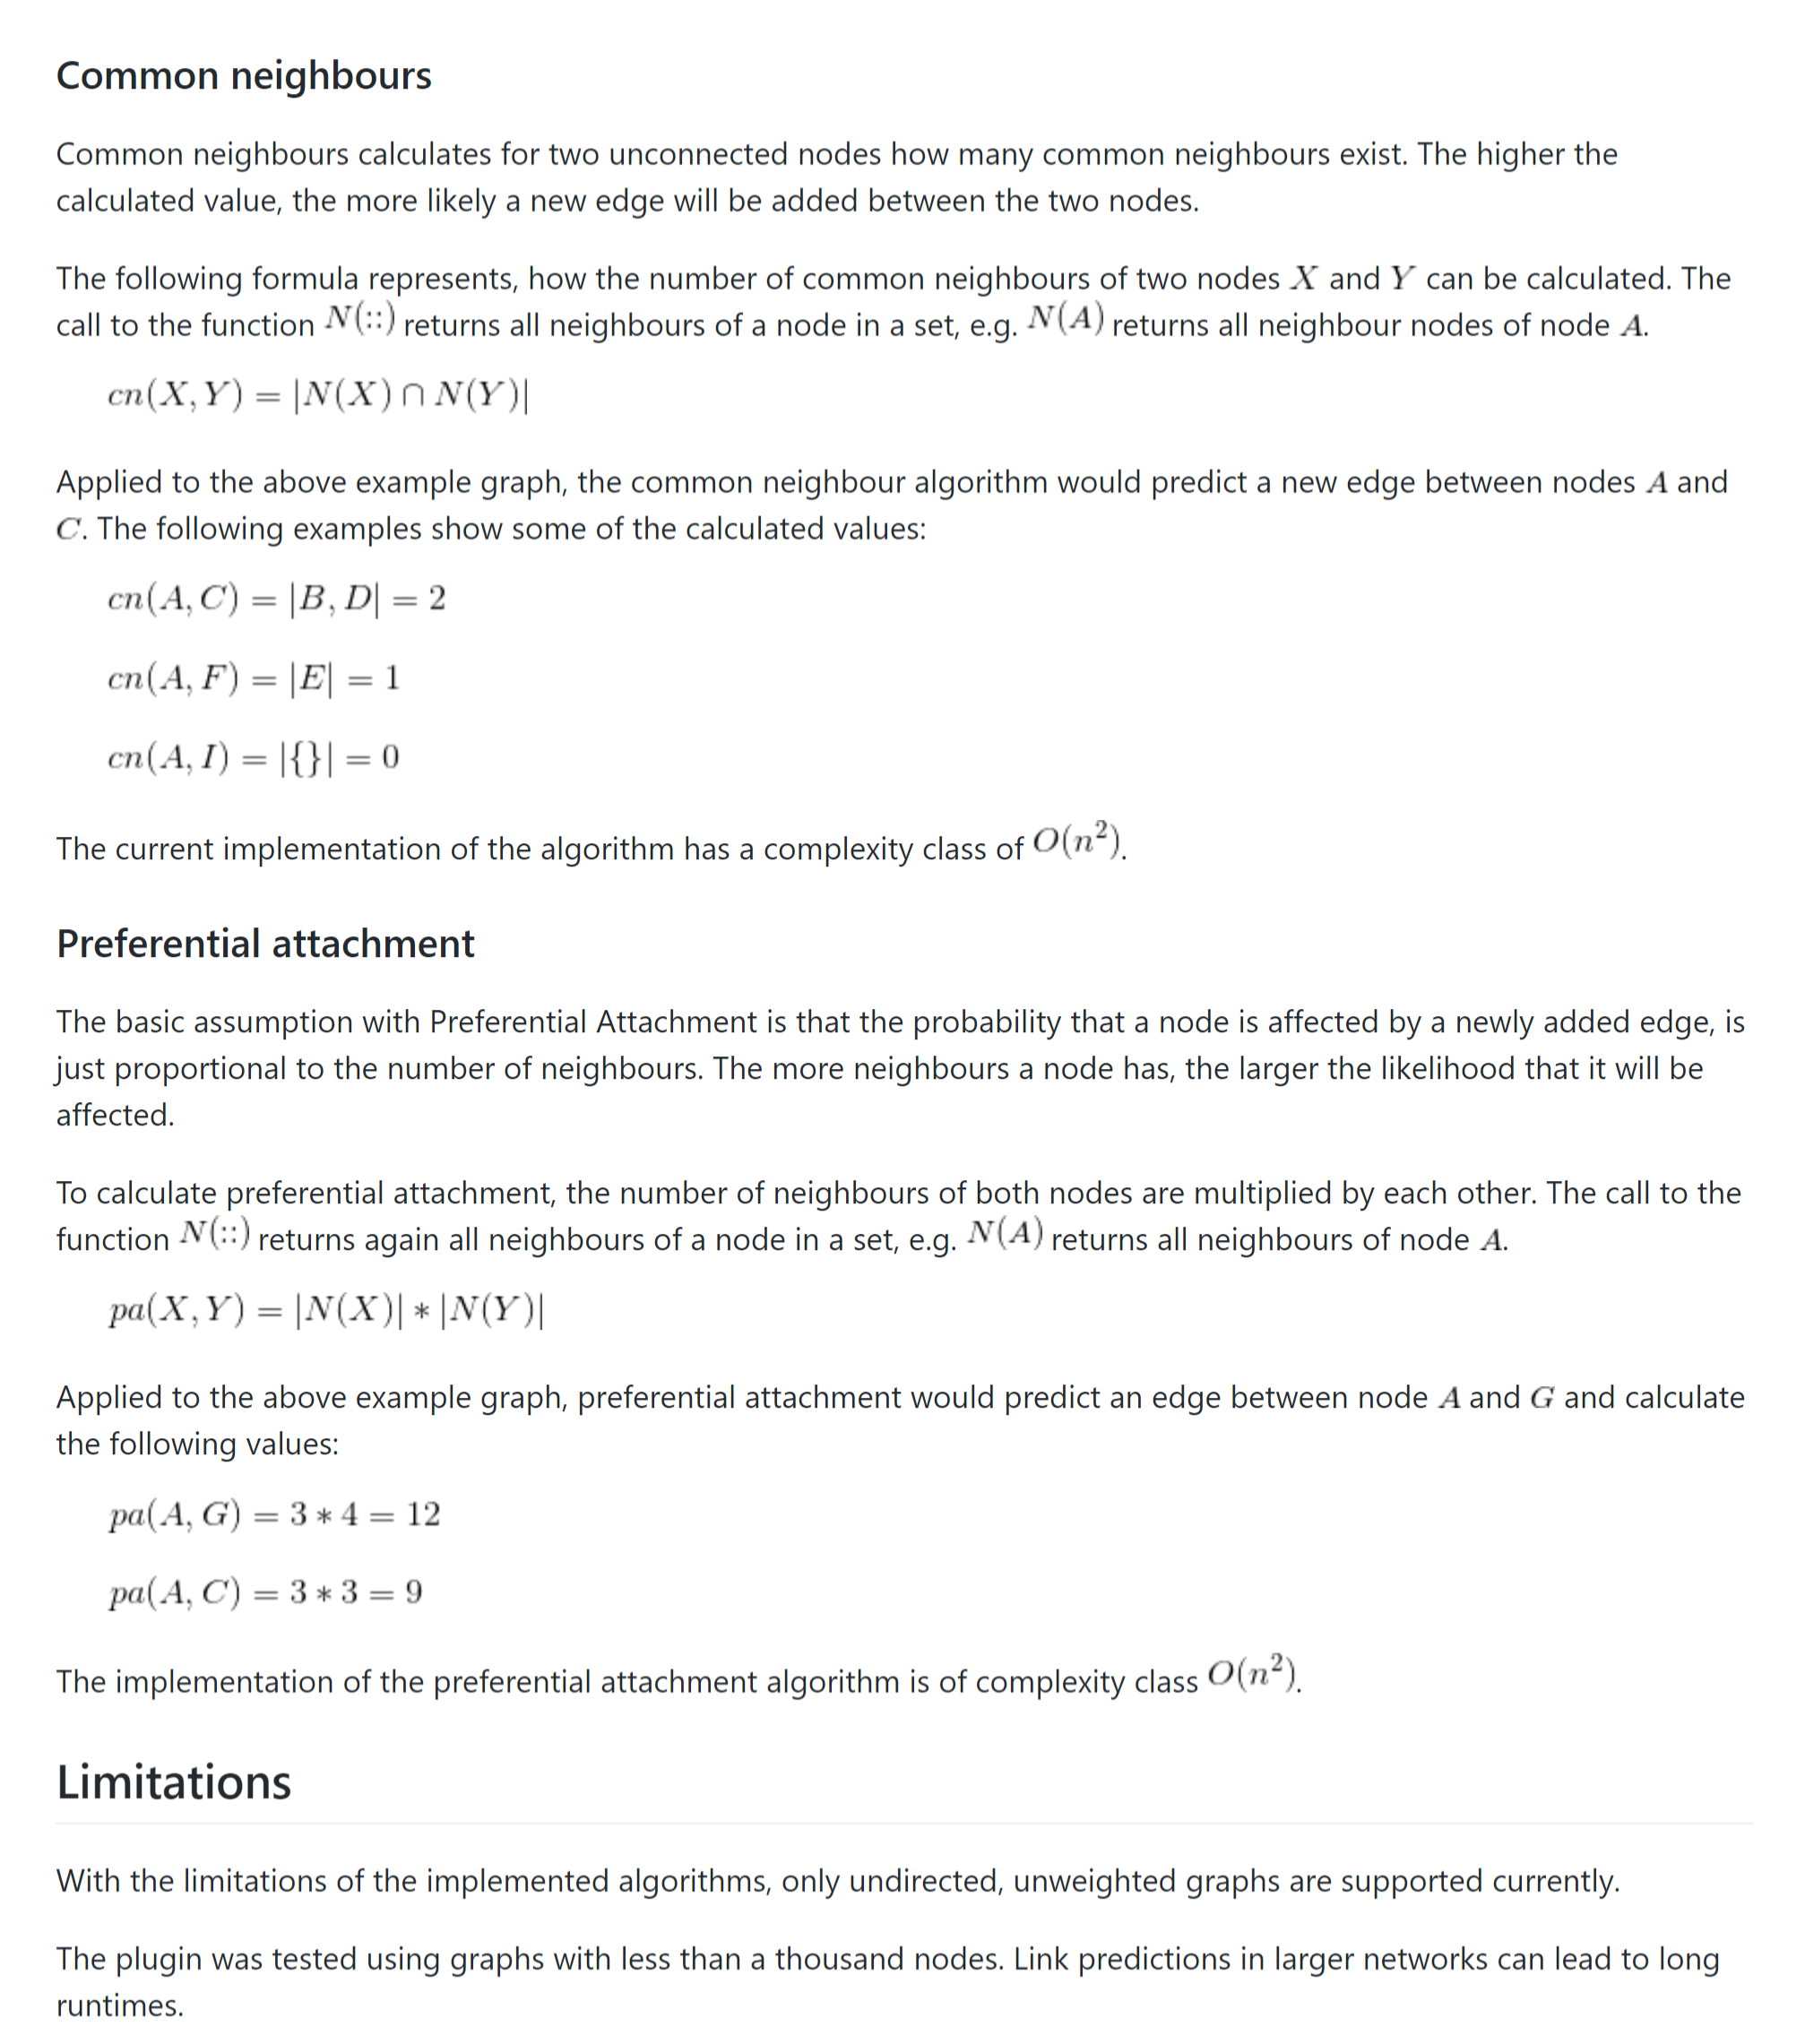
\includegraphics[width=\textwidth]{resources/readme_pt3.png}

\newpage

\section{Loggingkonzept}
\label{loggingkonzept}

Im Plugin wird das Logging-Framework log4j\footnote{https://logging.apache.org/log4j/2.x/} eingesetzt.
Das Logging wird eingesetzt um technische Probleme rückverfolgen zu können: Die Logs zeichnen Ereignisse auf, die für die Entwicklung und den Einsatz des Plugin von Nutzen sein können.
Insbesondere geht es darum ein Fehlverhalten der Applikation nachvollziehen und dokumentieren zu können.

\subsection{Logger erzeugen}
Logger sind für das Verfassen von Meldungen verantwortlich. Sie werden direkt aus dem Code aufgerufen und bestimmen mit Hilfe von Appendern wohin und in welchem Format die Meldungen geschrieben werden.
Für jede Klasse wird ein separater Logger erzeugt. Das Codelisting \ref{lstLoggerCreate} zeigt, wie ein solcher Logger in der gewünschten Klasse erzeugt wird.

\begin{lstlisting}[caption={Erzeugen eines Loggers},label=lstLoggerCreate]
    import org.apache.log4j.Logger;

    /**
     * ...
     */
    public class LinkPredictionStatistics \{

    // Console Logger
    private static Logger consoleLogger = LogManager.getLogger(LinkPredictionStatistics.class);
\end{lstlisting}

\subsection{Log-Einträge erzeugen}
%TODO: Add Log4j to Glossar
Log4j bietet verschiedene Log-Levels an, mit welchen Log-Einträge geschrieben werden können.
Tabelle \ref{tab_log_level} zeigt die verschiedenen Log-Levels anhand der \acs{API}-Docs von log4i:

\begin{table}[]
    \centering
    \resizebox{\textwidth}{!}{%
    \begin{tabular}{@{}ll@{}}
        \toprule
        Level & Beschreibung                                                                                                             \\ \midrule
        TRACE & The TRACE Level designates finer-grained informational events than the DEBUG                                             \\
        DEBUG & The DEBUG Level designates fine-grained informational events that are most useful to debug an application.               \\
        INFO  & The INFO level designates informational messages that highlight the progress of the application at coarse-grained level. \\
        WARN  & The WARN level designates potentially harmful situations.                                                                \\
        ERROR & The ERROR level designates error events that might still allow the application to continue running.                      \\
        FATAL & The FATAL level designates very severe error events that will presumably lead the application to abort.                  \\ \bottomrule
    \end{tabular}%
    }
    \caption{}
    \label{tab_log_levels}
\end{table}

Grundsätzlich kann direkt mit den Funktionen auf dem Logger-Objekt (z.B. \texttt{trace}, \texttt{debug}, etc.) geloggt werden.
Falls in der Log-Meldung Variabeln ausgewertet werden, empfiehlt sich jedoch die Lambda schreibweise mit Lazy-Evaluation.
Listing \ref{lstLoggerUse} zeigt zwei solcher Beispiele.

\begin{lstlisting}[caption={Log-Einträge erzeugen},label=lstLoggerUse]
    public int getNextIteration(Graph graph, String algorithm) {
        consoleLogger.trace("Lookup next iteration");
        int lastIteration;
        // do some lookups here

        consoleLogger.log(Level.DEBUG, () -> "Number of last iteration: " + lastIteration);
    }
\end{lstlisting}

\subsection{Logger Hierarchie}
Alle Logger der verschiedenene Klassen erben vom Root-Logger. Über diesen kann die Konfiguration für alle Logger geändert werden.
Einzelne Logger können die Root-Konfiguration bei Bedarf übersteuern.

\subsection{Appender}
Aktuell wird im Plugin hautpsächlich der \texttt{ConsoleAppender} eingesetzt.
Mit dessen Hilfe kann direkt in die Gephi-Konsole geloggt werden.

\subsection{Konfiguration}

\begin{lstlisting}[caption={log4j.xml},label=lstLoggerCreate]
<?xml version="1.0" encoding="UTF-8" ?>
<Configuration>
    <Appenders>
    <Console name="console" target="SYSTEM_OUT">
    <PatternLayout pattern="%d{HH:mm:ss} %-5p %L [%C] - %m%n"/>
    </Console>

    <Loggers>
        <Logger name = "org.gephi.plugins.linkprediction.statistics.PreferentialAttachmentStatistics" additivity="false">
            <AppenderRef ref="console" />
        </Logger>

        <Root level="INFO" additivity="false">
            <AppenderRef ref="file" />
        </Root>
    </Loggers>

</Configuration>
\end{lstlisting}

\section{Exception-Handling}
\label{exceptionhandling}


